\section{Masking}

\begin{frame}
    \sectionpage
\end{frame}

\begin{frame}{Side Channel Attacks}
    Implementations of theoretically secure cryptosystems may \textit{leak} some information, allowing an 
    attacker to extract secret data.
    \begin{block}{Side Channel Vulnerabilities}
        Side channel attacks take use of different leakage sources, such as:
        \begin{itemize}
            \item Execution time
            \item Power consumption
            \item Electromagnetic radiation
            \item Differential faults
        \end{itemize}
    \end{block}
\end{frame}

\begin{frame}{Power Analysis}
    \begin{block}{Simple Power Analysis}
        Analyze the electrical current drawn by the device over time: different operations may have different power consumption.
    \end{block}
    \begin{block}{Differential Power Analysis}
        Statistically analyze the power consumption of the device over different executions: detect biases between, for example, a known secret key and a unknown one.
    \end{block}
\end{frame}

\begin{frame}{Power Analysis}
    \begin{figure}
        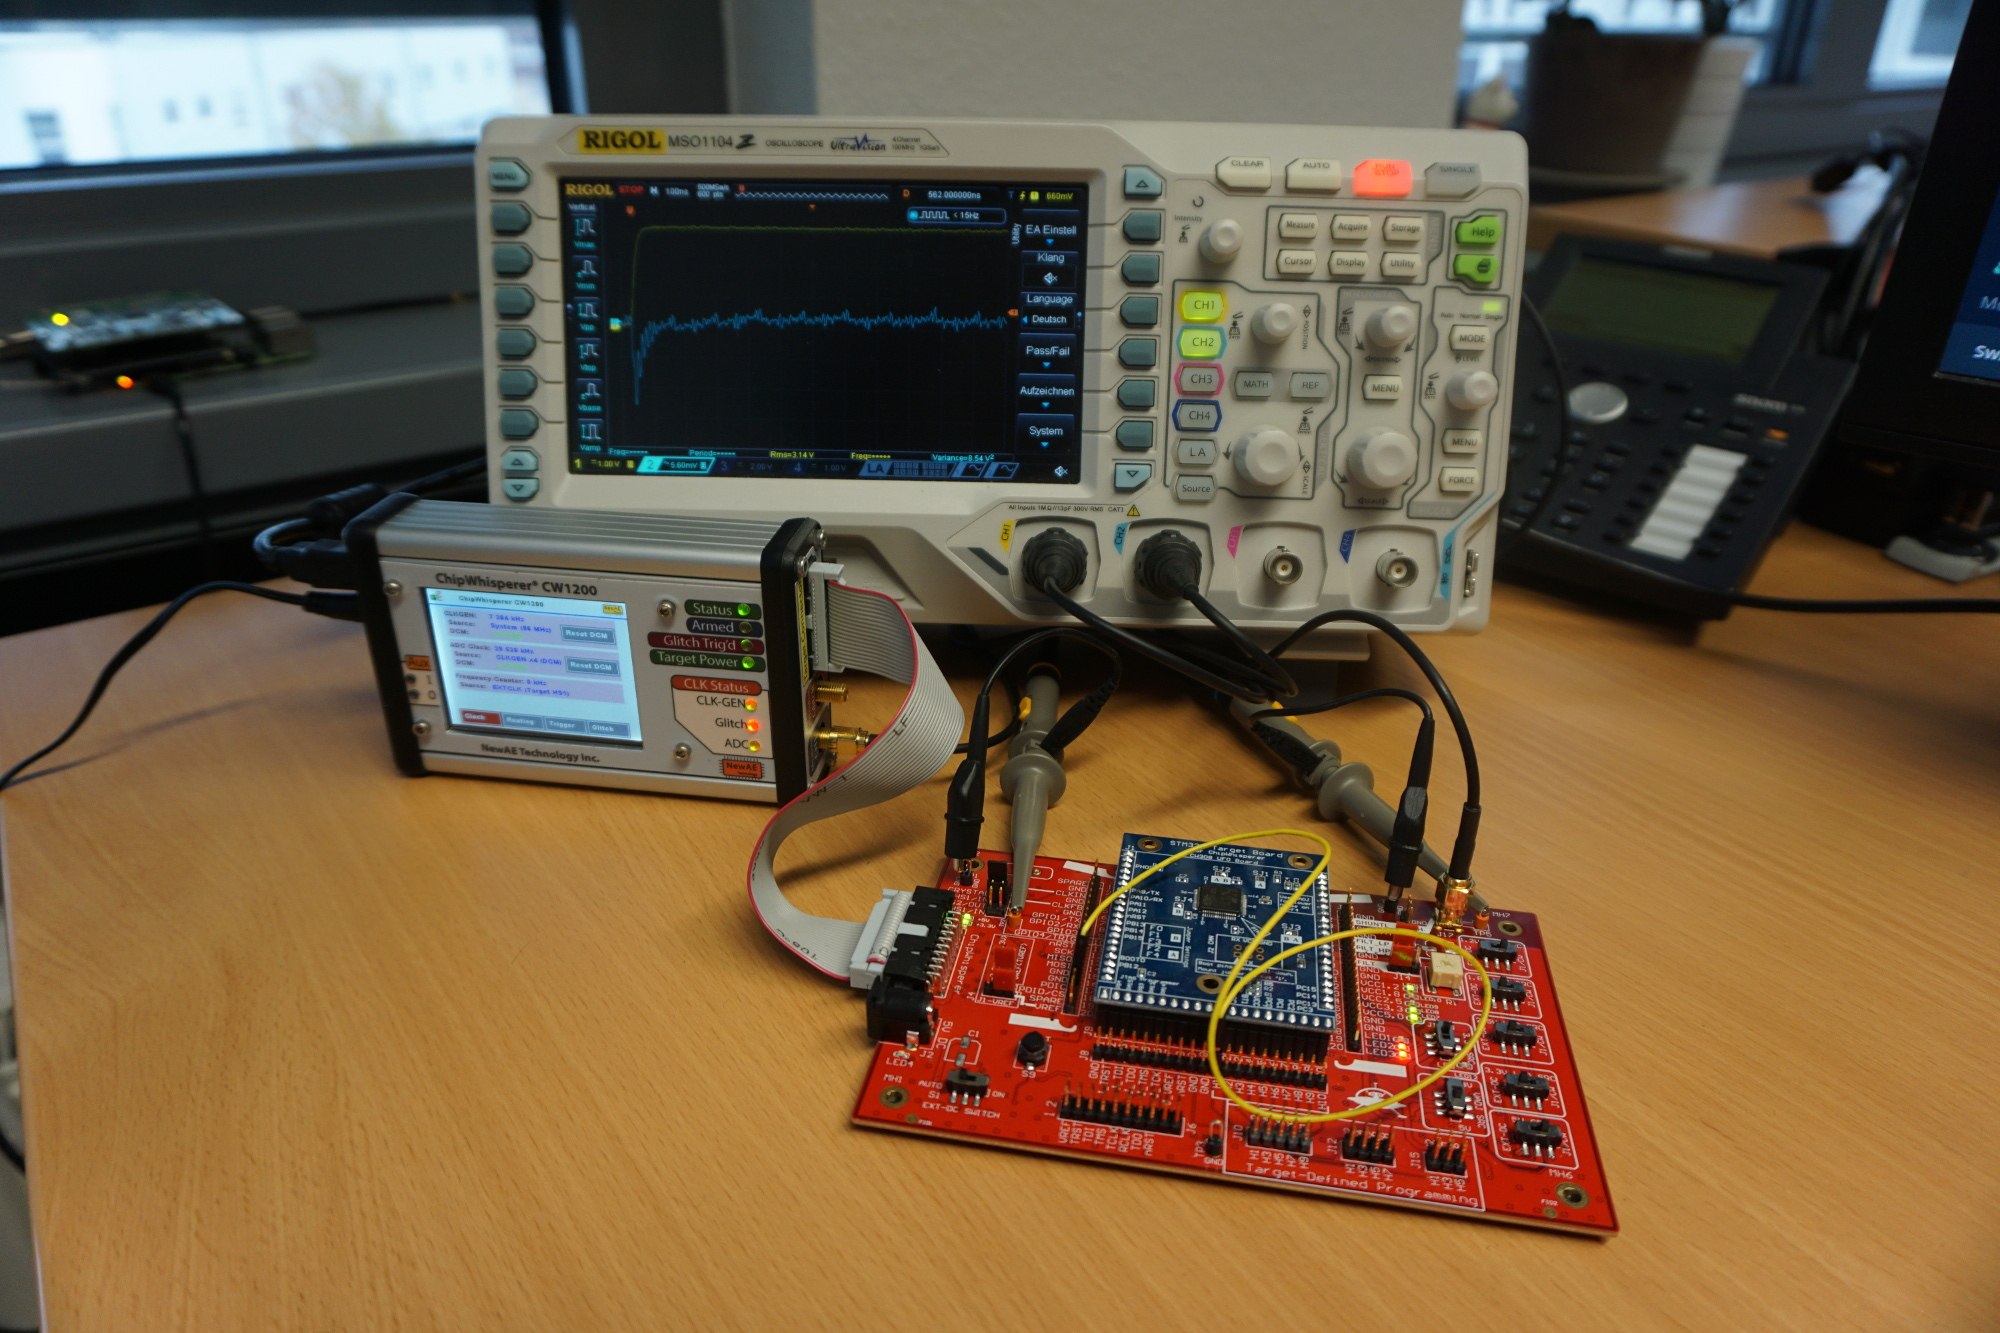
\includegraphics[scale=0.6]{images/chipwhisperer_with_target_and_oscilloscope.jpg}
        \caption{ChipWhisperer}
        % \footnote{https://www.schutzwerk.com/en/43/posts/poweranalysis\_1/}
    \end{figure}
    
\end{frame}

\begin{frame}{Countermeasures to Power Analysis}
    Power analysis attacks are usually passive, so they cannot be detected by the device.
    \begin{block}{}
        To mitigate the effectiveness of these attacks, it is possible to:
        \begin{itemize}
            \item \textbf{SPA}: avoid branches with conditions that depend on secret data
            \item \textbf{DPA}: \textit{mask} the secret data when performing operations on them
        \end{itemize}
    \end{block}
    \begin{block}{Masking}
        Given a secret $x$, we can split it into $d$ \textit{shares} in such a way that
        \begin{equation*}
            x = x_0 \odot x_1 \cdots \odot x_{d-1}
        \end{equation*}
        for some operation $\odot$ (e.g. XOR in binary fields).
    \end{block}
\end{frame}

\begin{frame}{Securing AND gates}
    \begin{block}{Probing Model~\cite{ishai2003private}}
        Given an algorithm that operates on data split among $d$ shares, we say that the algorithm is 
        secure against a $(d-1)$-th order probing attack if, on input $x = (x_1, \cdots, x_d)$, it admits no
        tuple of $d-1$ (or less) shares that depends on $x$
    \end{block}
    \begin{block}{Ishai-Sahai-Wagner’s Scheme}
        Let $x = (x_1, \cdots, x_d), y = (y_1, \cdots, y_d)$ binary variables: to securely compute $x \wedge y$ at order $\lfloor d/2 \rfloor$:
        \begin{itemize}
            \item Pick a random bit $r_{i, j}$
            \item Compute $r_{j, i} = (r_{i, j} + (x_i \wedge y_j)) + (x_j \wedge y_i)$
            \item Compute $c_i = (x_i \wedge y_j) + \sum_{j \neq i} r_{i, j}$ 
        \end{itemize}
    \end{block}
\end{frame}

\begin{frame}{Securing multiplications}
    The ISW scheme can be extended from $\mathds{F}_2$ to $\mathds{F}_2^{n}$, increasing its security to $d$-th order attacks
    \begin{block}{Rivain-Prouff's Scheme}
        Let $a = (a_1, \cdots, a_d), b = (b_1, \cdots, b_d)$, with $ a_i, b_i \in \mathds{F}_2^n$
        \begin{itemize}
            \item Calculate $c_i \leftarrow a_i\cdot b_i$ for each share
        \end{itemize}
        For $i$ from 1 to $d$ and $j$ from $i+1$ to $d$:
        \begin{itemize}
            \item Extract a random value $s \xleftarrow{\$} \mathds{F}_2^n$
            \item Calculate $s^{'} \leftarrow (s + (a_i \cdot b_j)) + (a_j \cdot b_i)$
            \item Calculate $c_i \leftarrow c_i + s$ and  $c_j \leftarrow c_j + s^{'}$ 
        \end{itemize}
        The sum of the shares $(c_1, \cdots, c_d)$ yields the product $a\cdot b$
    \end{block}
\end{frame}